\documentclass{beamer}
\usetheme{CambridgeUS}
\usecolortheme{dolphin}
\usepackage{hyperref}
\usepackage{multimedia}
\usepackage{biblatex}

% set colors
\definecolor{myNewColorA}{RGB}{126,12,110}
\definecolor{myNewColorB}{RGB}{165,85,154}
\definecolor{myNewColorC}{RGB}{203,158,197}
\setbeamercolor*{palette primary}{bg=myNewColorC}
\setbeamercolor*{palette secondary}{bg=myNewColorB, fg = white}
\setbeamercolor*{palette tertiary}{bg=myNewColorA, fg = white}
\setbeamercolor*{titlelike}{fg=myNewColorA}
\setbeamercolor*{title}{bg=myNewColorA, fg = white}
\setbeamercolor*{item}{fg=myNewColorA}
\setbeamercolor*{caption name}{fg=myNewColorA}

\title{Fúziós energia egy új megközelítése}
\subtitle{Helion}
\author[Péter Bence]{Péter Bence Gábor\\X89O8X}
\institute{Széchenyi István Egyetem}
\date{2023. Május 9.}

\begin{document}
\titlepage


\begin{frame}
    \frametitle{Tartalom}
    \tableofcontents
\end{frame}


\section{Bevezetés}
\begin{frame}
    \frametitle{Bevezetés \hyperlink{1}{\small[1]}}
    \begin{itemize}
        \item Nap magja
        \begin{itemize}
            \item Hőmérséklet: 15 millió Kelvin
            \item Nyomás: 265 milliárd bar
        \end{itemize}
    \end{itemize}
    \begin{figure}
        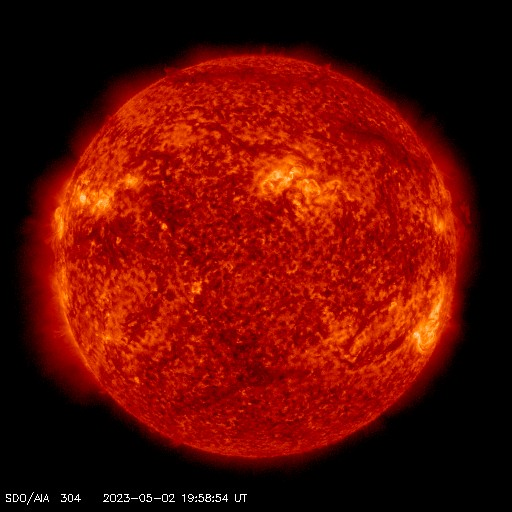
\includegraphics[scale=0.30]{latest_512_0304.jpg}
        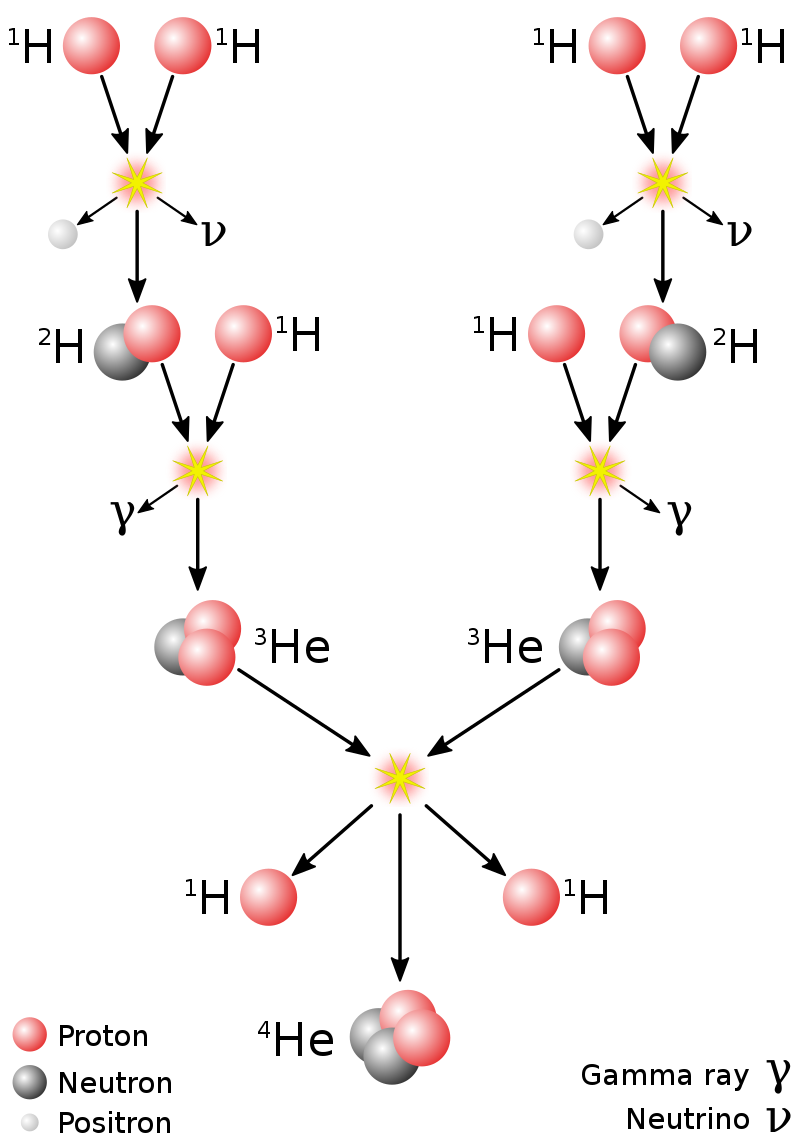
\includegraphics[scale=0.13]{800px-Fusion_in_the_Sun.svg.png}
    \end{figure} 
\end{frame}


\subsection{Fúzió}
\begin{frame}
    \frametitle{Fúzió \hyperlink{2}{\small[2]}}
    \begin{figure}
        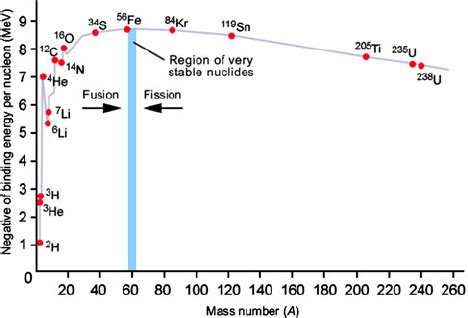
\includegraphics[scale=0.6]{fusion_fission.jpeg}
    \end{figure} 
\end{frame}


\subsection{Tokamak}
\begin{frame}
    \frametitle{Tokamak \hyperlink{3}{\small[3]}}
    \begin{columns}
        \column{0.4\textwidth}
        \begin{itemize}
            \item Nagy sebességű neutronok
            \item 17.6 MeV
        \end{itemize}
        \column{0.6\textwidth}
        \begin{figure}
            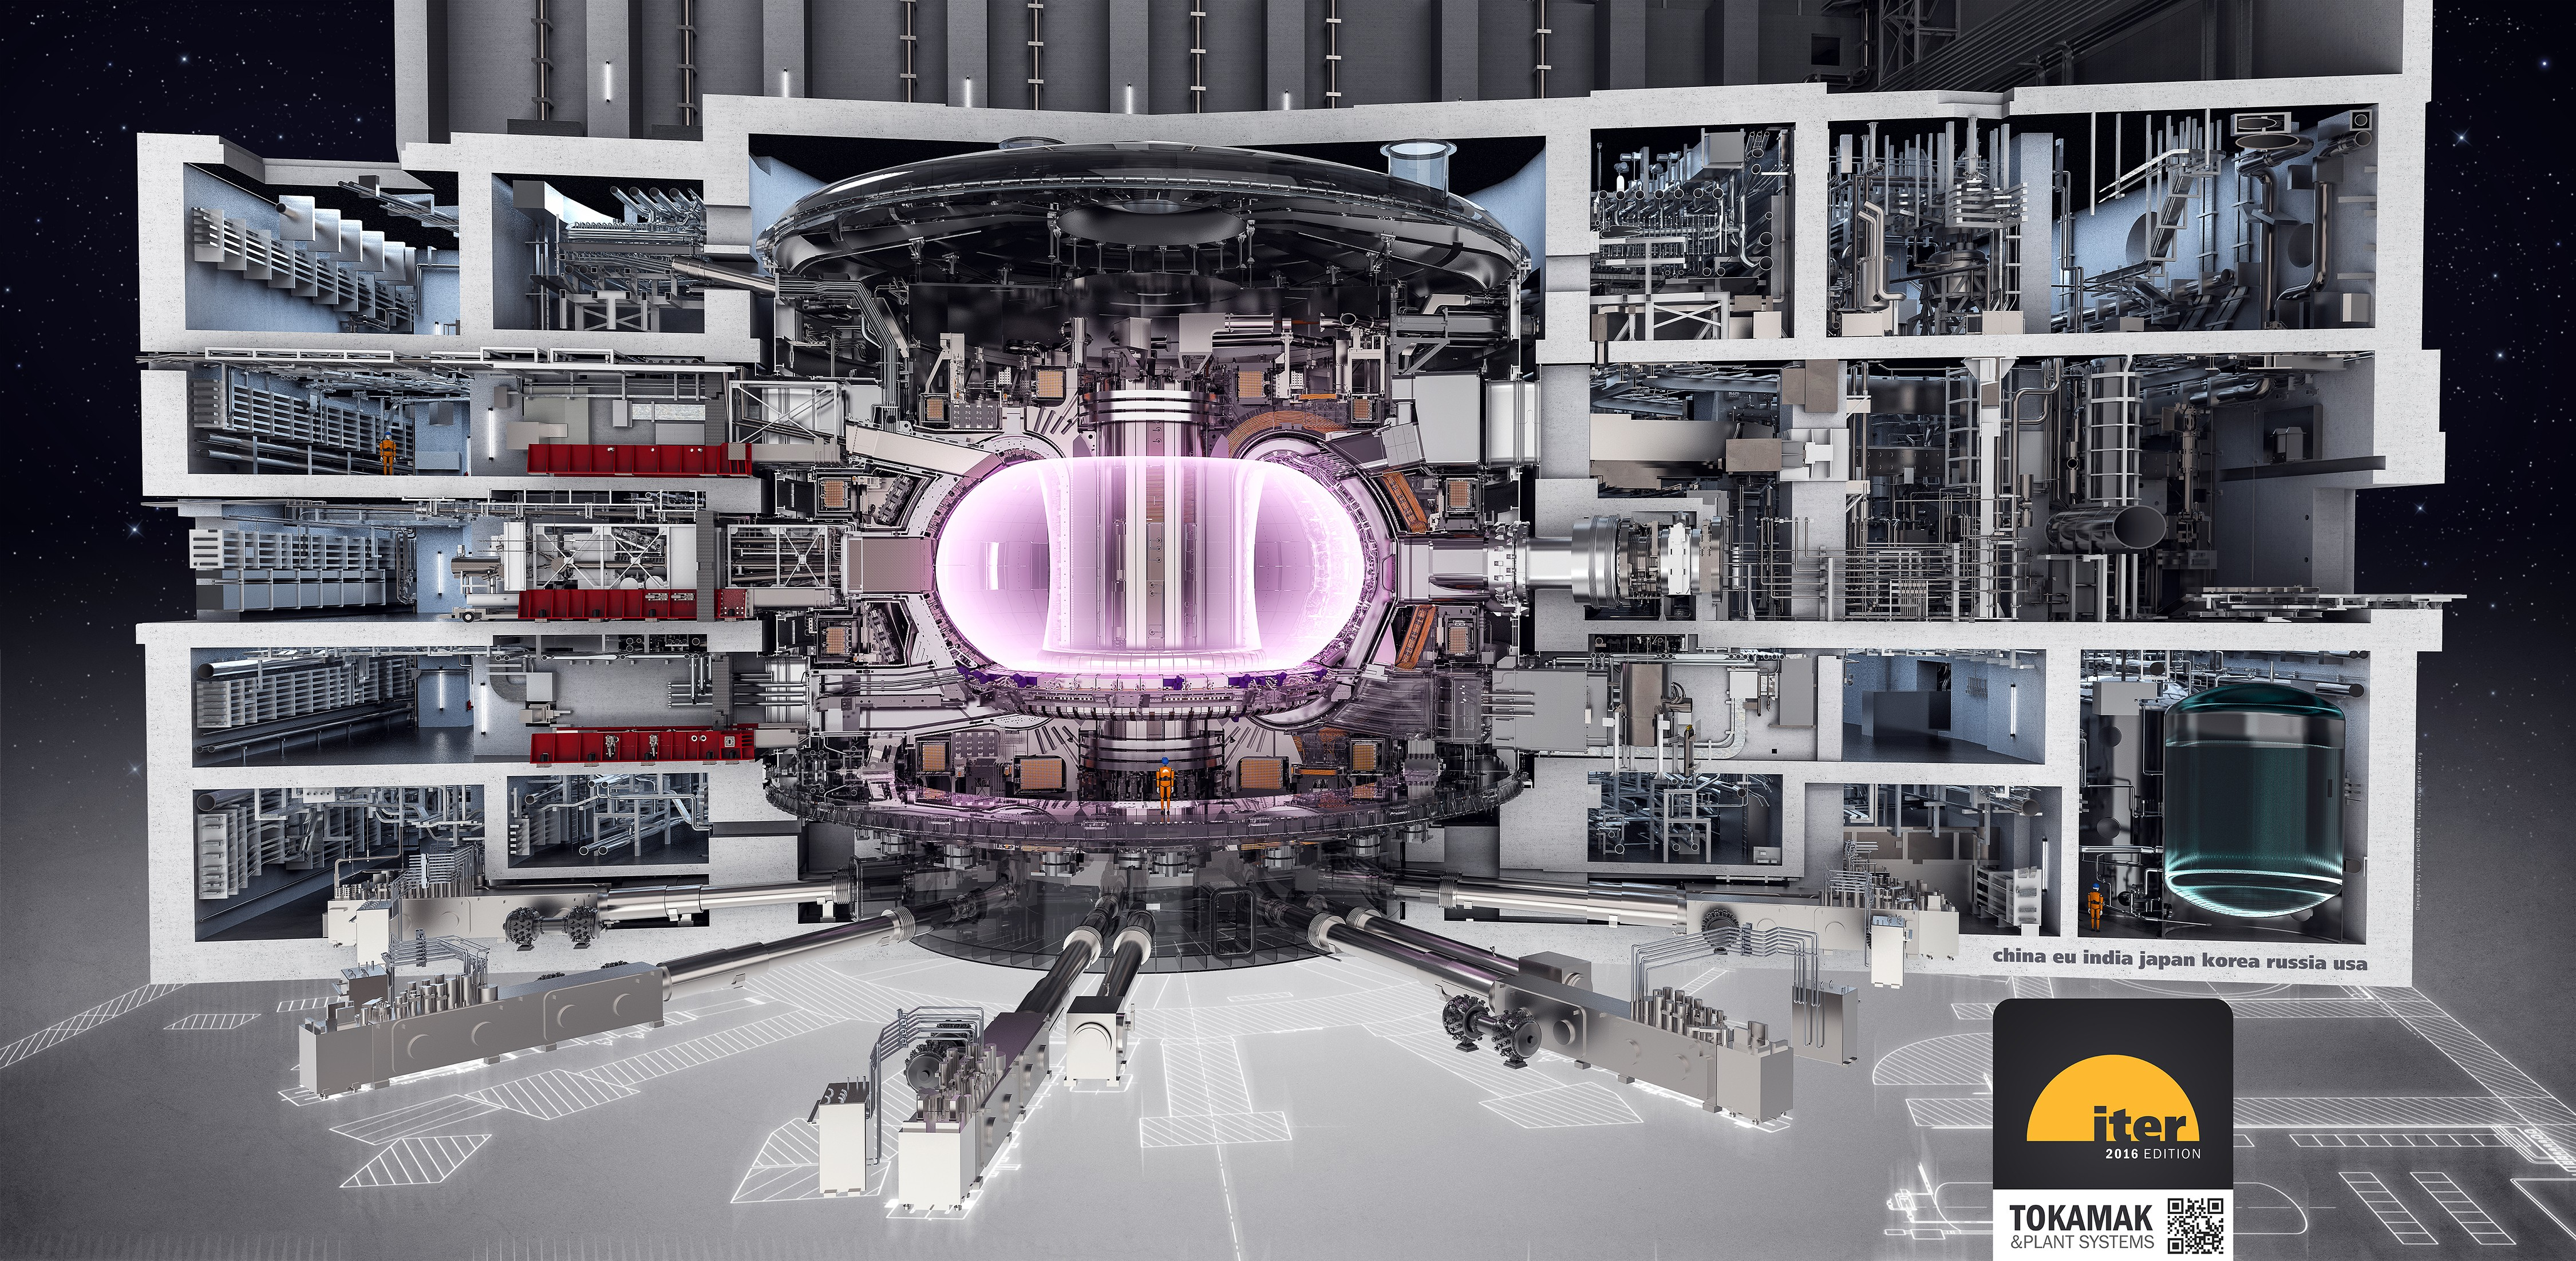
\includegraphics[scale=0.043]{iter.jpeg}
            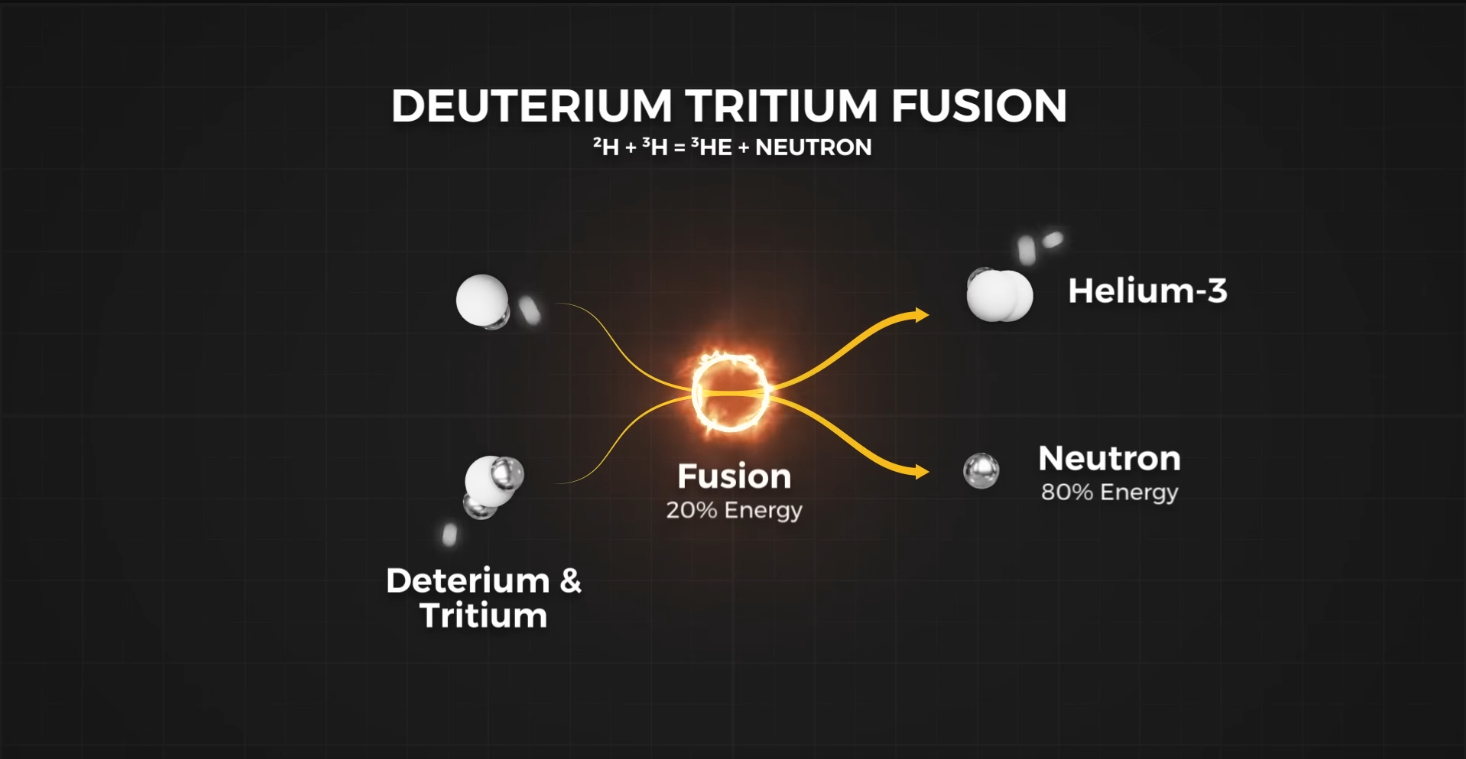
\includegraphics[scale=0.135]{deut_trit_v2.png}
        \end{figure}  
    \end{columns}
   
\end{frame}


\section{Helion}
\begin{frame}
    \frametitle{Helion \hyperlink{4}{\small[4]}\hyperlink{5}{\small[5]}}
    \begin{columns}
        \column{0.3\textwidth}
        \begin{itemize}
            \item Magán cég az USA-ban
            \item Alapítvás éve: 2013
            \item CEO: Dr. David Kirtley
            \item Legújabb prototípus: Trenta
        \end{itemize}
        \column{0.7\textwidth}
        \begin{figure}
            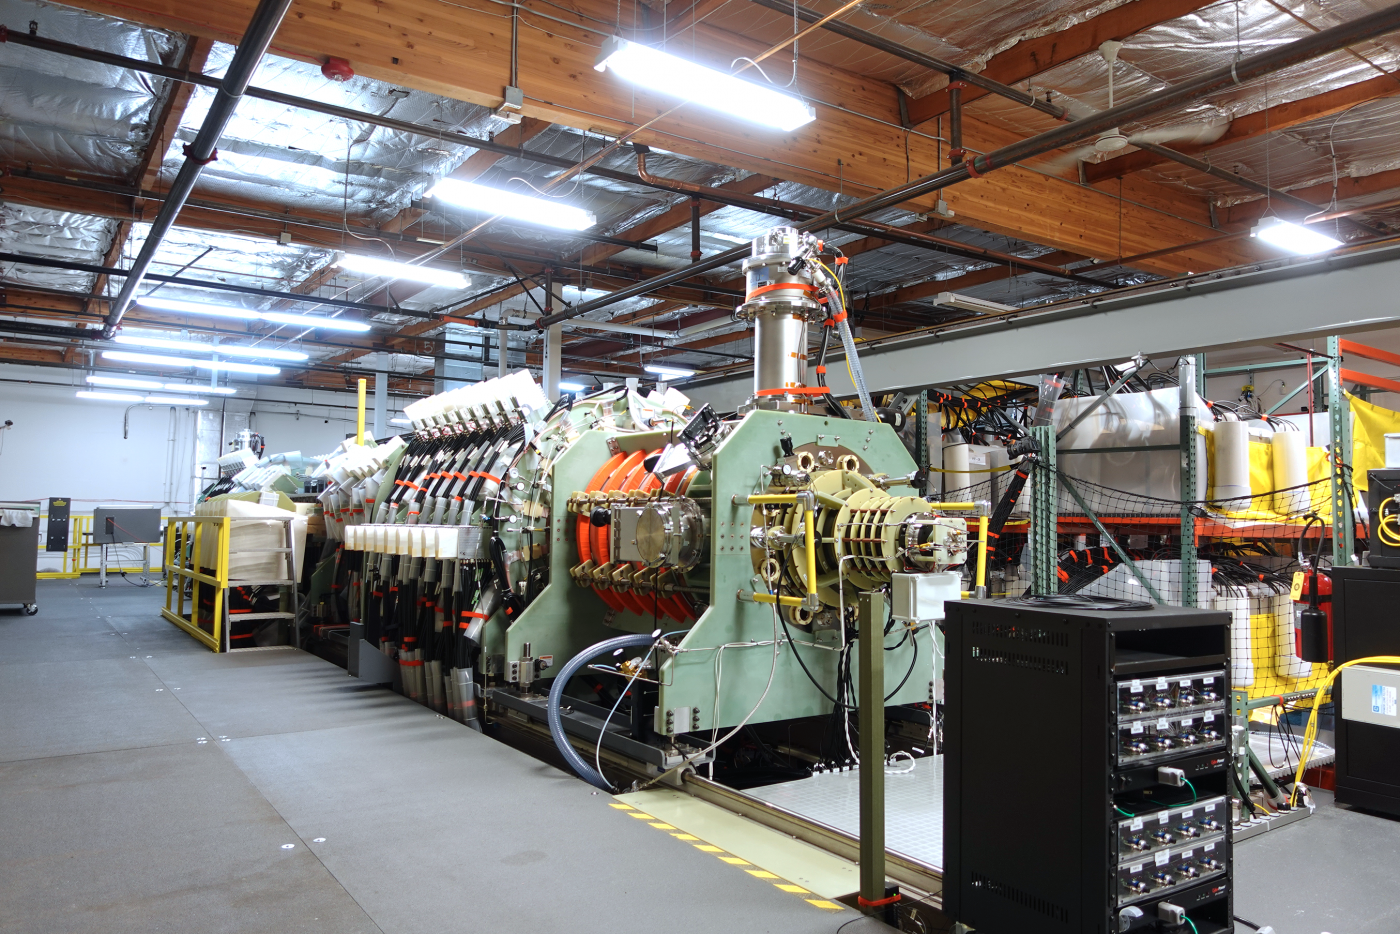
\includegraphics[scale=0.2]{trenta-1-1400x934.png}
        \end{figure}    
    \end{columns}
\end{frame}

\subsection{Működési elv}
\begin{frame}
    \frametitle{Működési elv}
    \begin{columns}
        \column{0.3\textwidth}
        \begin{itemize}
            \footnotesize
            \item Elektromágnes
            \item Tekercsenként $10^5A$
            \item Kondenzátorok: 
            \begin{itemize}
                \item kJ nagyságú energiamennyiség
                \item kisütés pár $\mu s$ alatt
            \end{itemize}
            \item Cél: másodpercenkénti több ismétlés
        \end{itemize}
        \column{0.7\textwidth}
        \movie[showcontrols=true, loop=true]{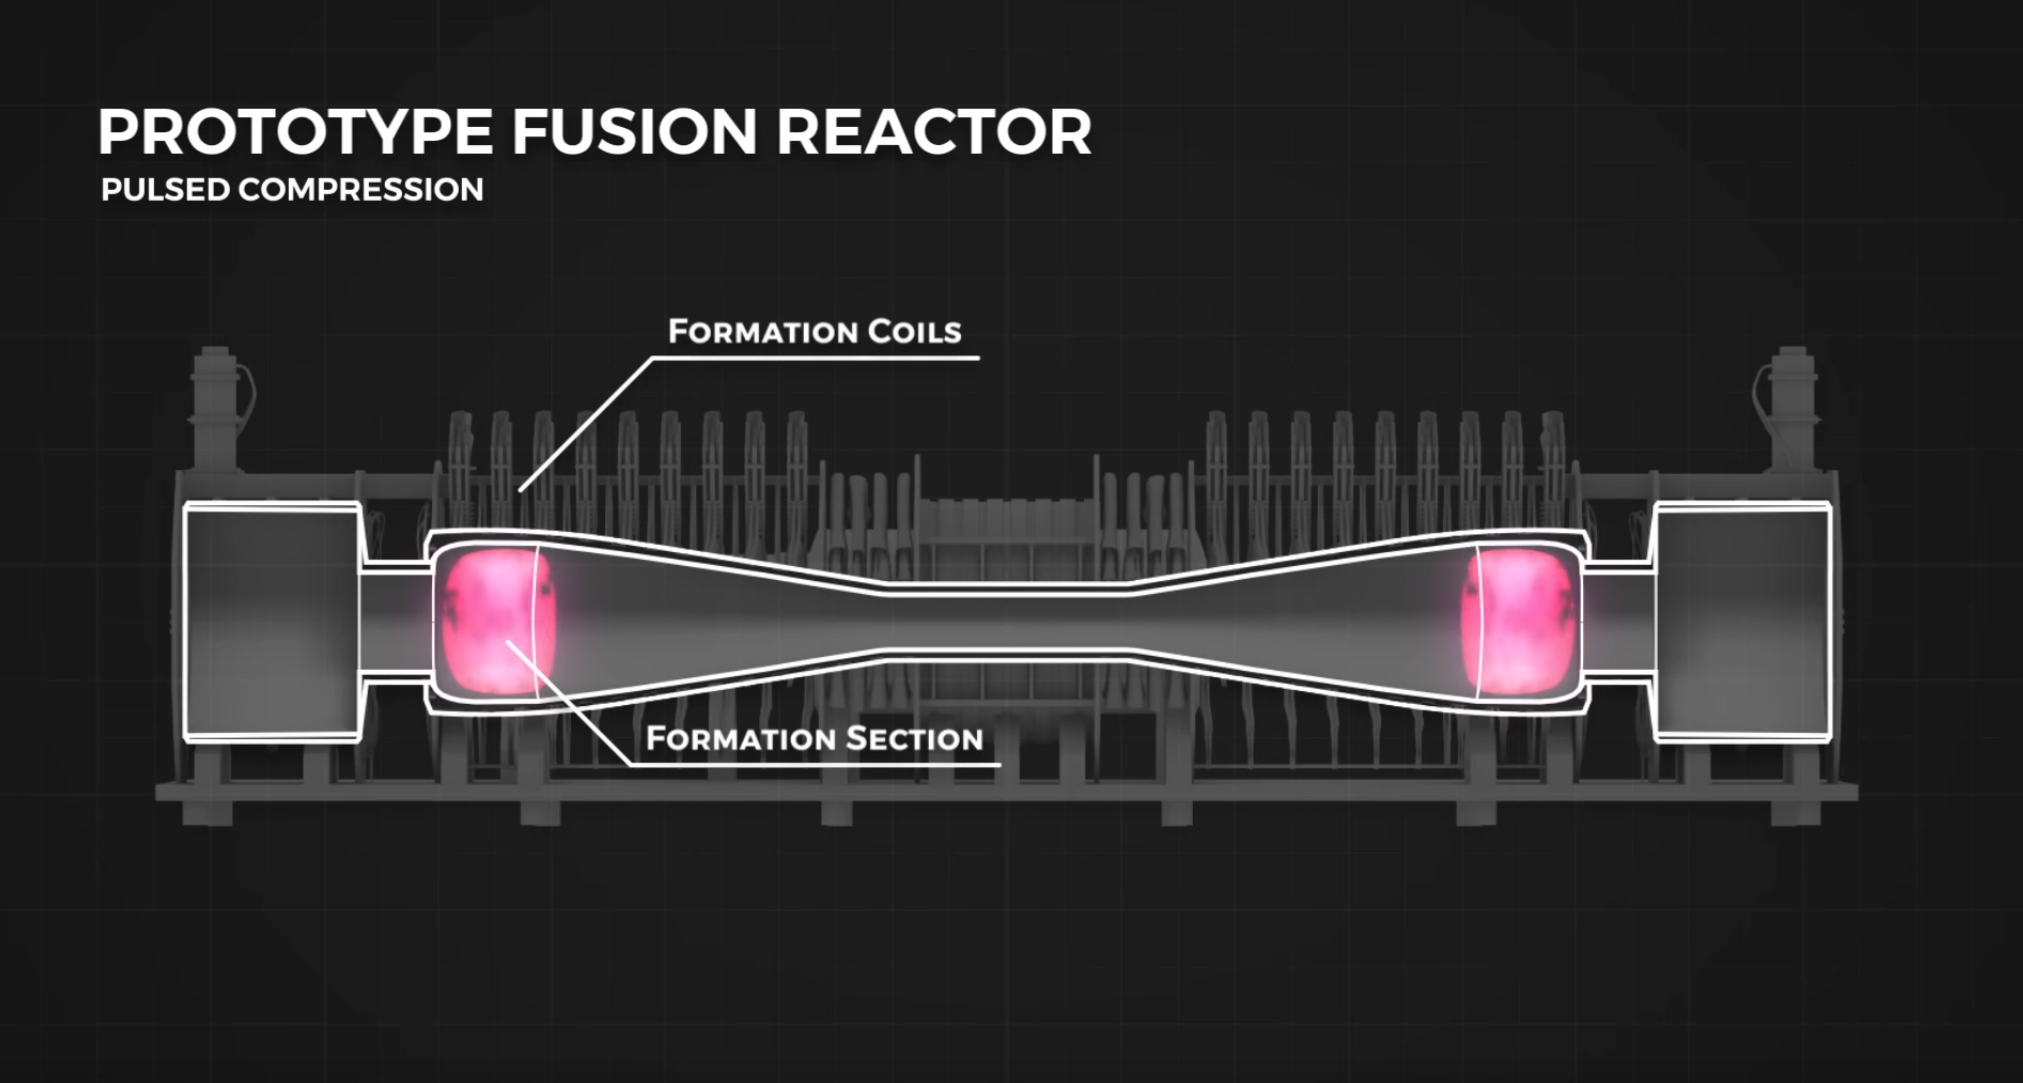
\includegraphics[scale=0.11]{helion_fusion_thumbnail.png}}{helion_fusion_video.mp4}   
    \end{columns}
\end{frame}
\begin{frame}
    \frametitle{Field-Reversed Configuration (FRC) \hyperlink{6}{\small[6]}}
    \begin{itemize}
        \item Tórusz alak
        \item Plazma egybetartása
        \item Kezdeti ionizálás: Neutral-beam injection \hyperlink{7}{\small[7]}
    \end{itemize}
    \begin{figure}
        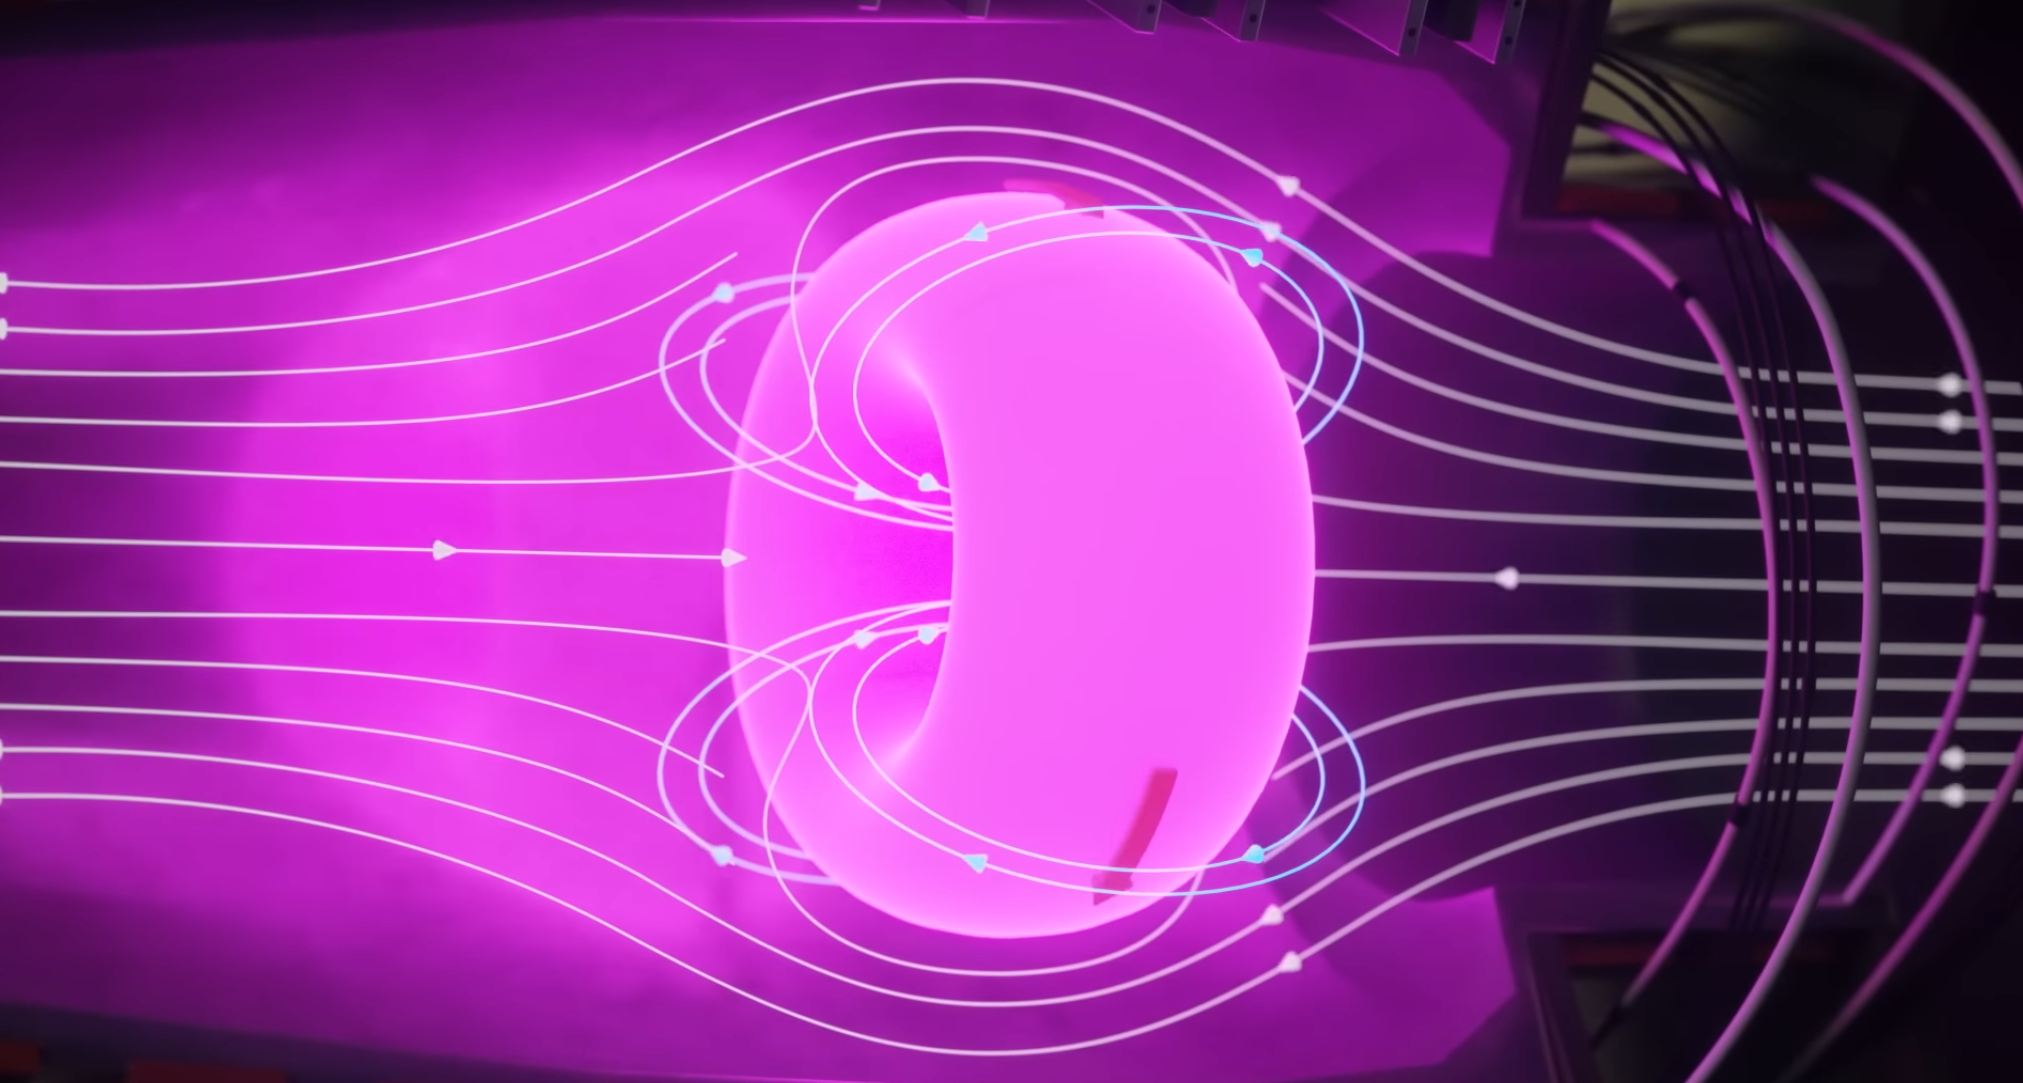
\includegraphics[scale=0.15]{field_reverse_config.png}
    \end{figure}
\end{frame}
\begin{frame}
    \frametitle{Fúzió elérése}
    \begin{itemize}
        \item Középen találkozó FRC-k
        \item Plazma nyomás és Elektromágneses nyomás aránya magas: $\beta \approx 1$ \hyperlink{8}{\small[8]}\hyperlink{9}{\small[9]}
        \item Elért hőmérséklet: $10^8K$
    \end{itemize}
    \begin{figure}
        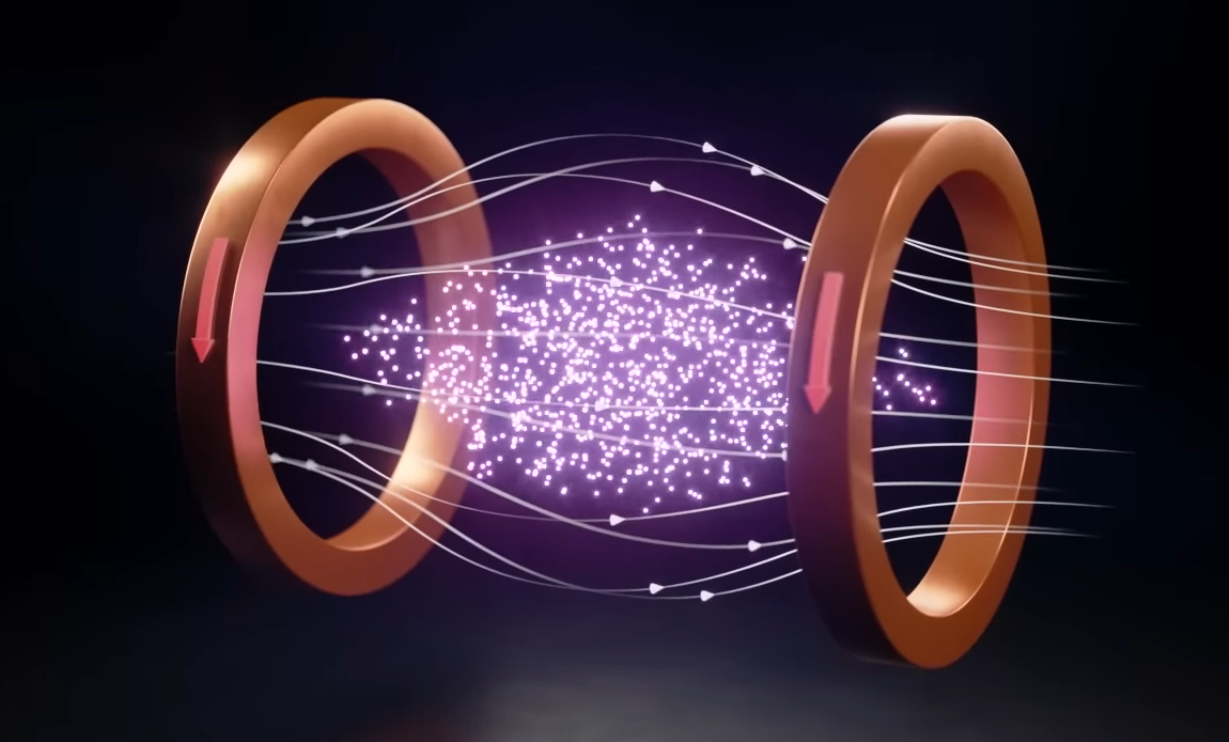
\includegraphics[scale=0.2]{piston.png}
    \end{figure}
\end{frame}

\subsection{Üzemanyag}
\begin{frame}
    \frametitle{Deuterium + Deuterium fúzió}
    \begin{columns}
        \column{0.5\textwidth}
        \begin{figure}
            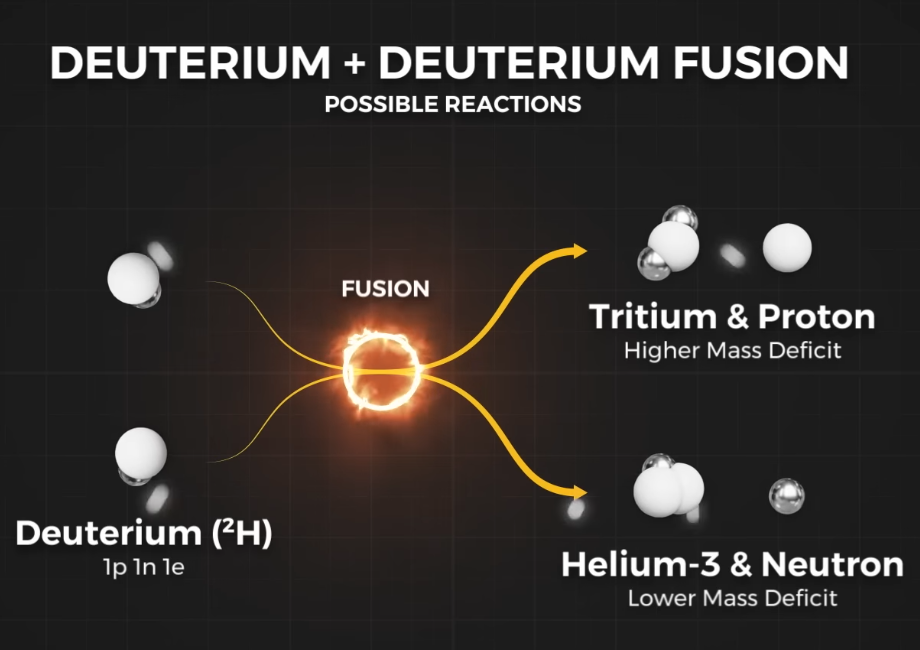
\includegraphics[scale=0.2]{d_d_fusion_v2.png}
        \end{figure}   
        \column{0.5\textwidth}
        \begin{figure}
            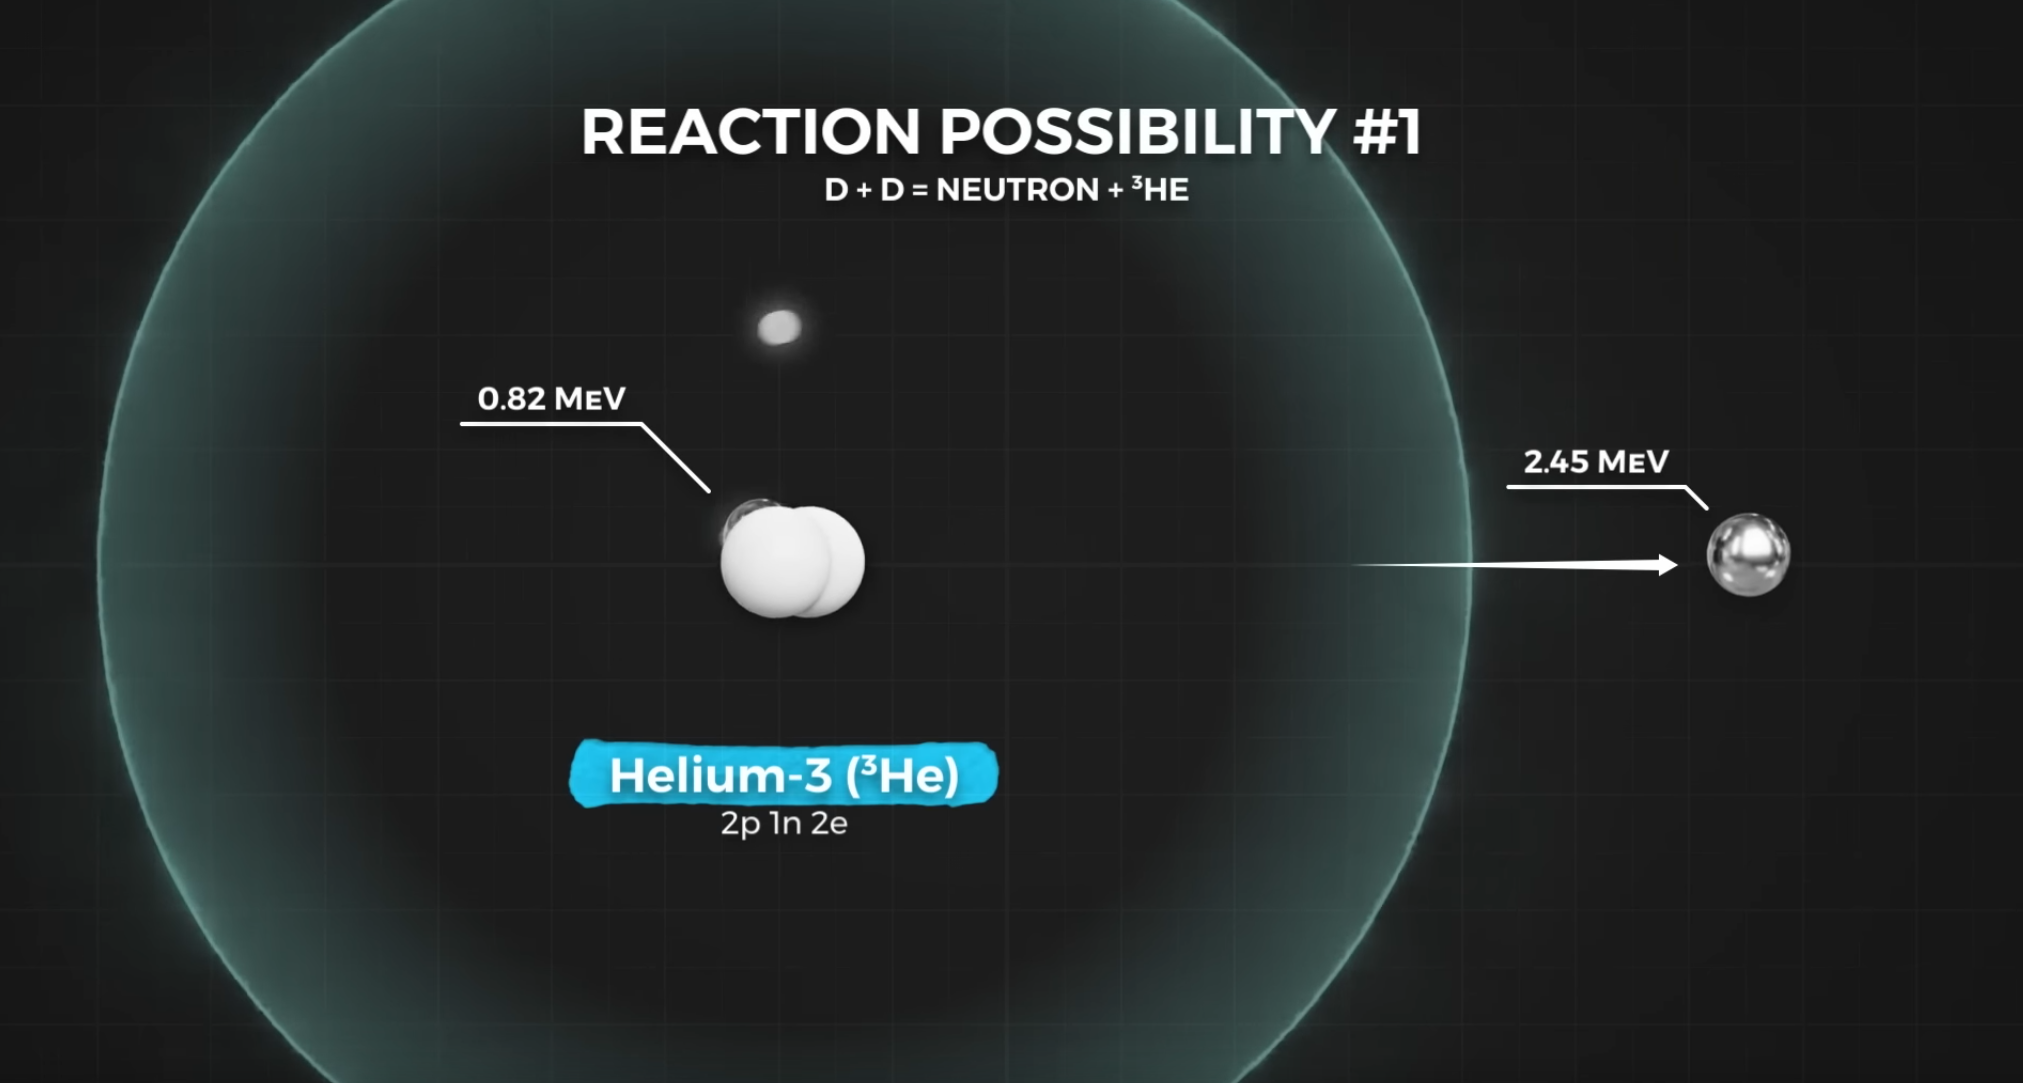
\includegraphics[scale=0.08]{d_d_fusion_possibility_1.png}
            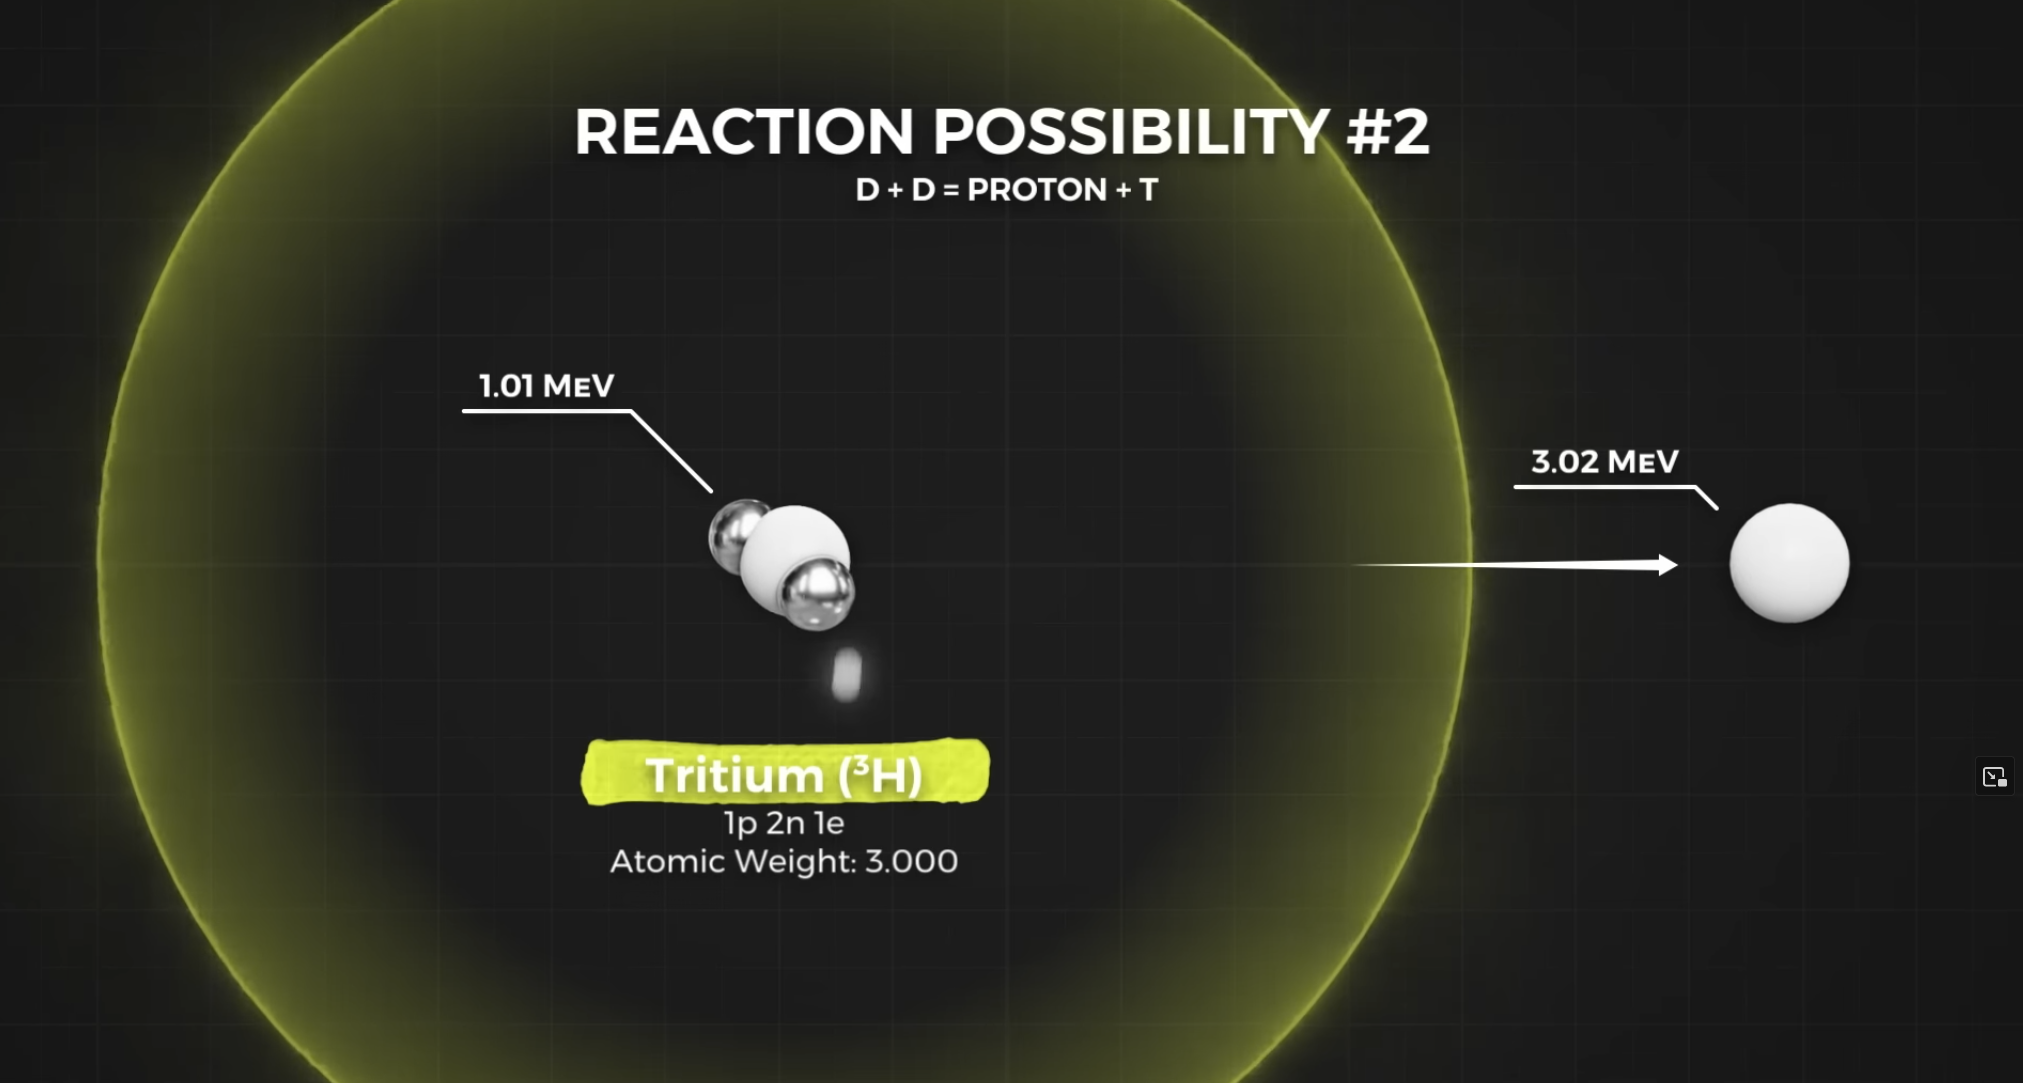
\includegraphics[scale=0.08]{d_d_fusion_possibility_2.png}
        \end{figure}   
    \end{columns}
\end{frame}
\begin{frame}
    \frametitle{Deuterium + Helium-3 fúzió \hyperlink{10}{\small[10]}\hyperlink{11}{\small[11]}}
    \begin{columns}
        \column{0.4\textwidth}
        \begin{itemize}
            \item Magas Plasma-Beta lehetővé teszi a D-He-3 fúziót
            \item Aneutronic fusion: gyorsan mozgó pozitív töltésú részecskék
            \item 18.3 MeV
        \end{itemize}
        \column{0.6\textwidth}
        \begin{figure}
            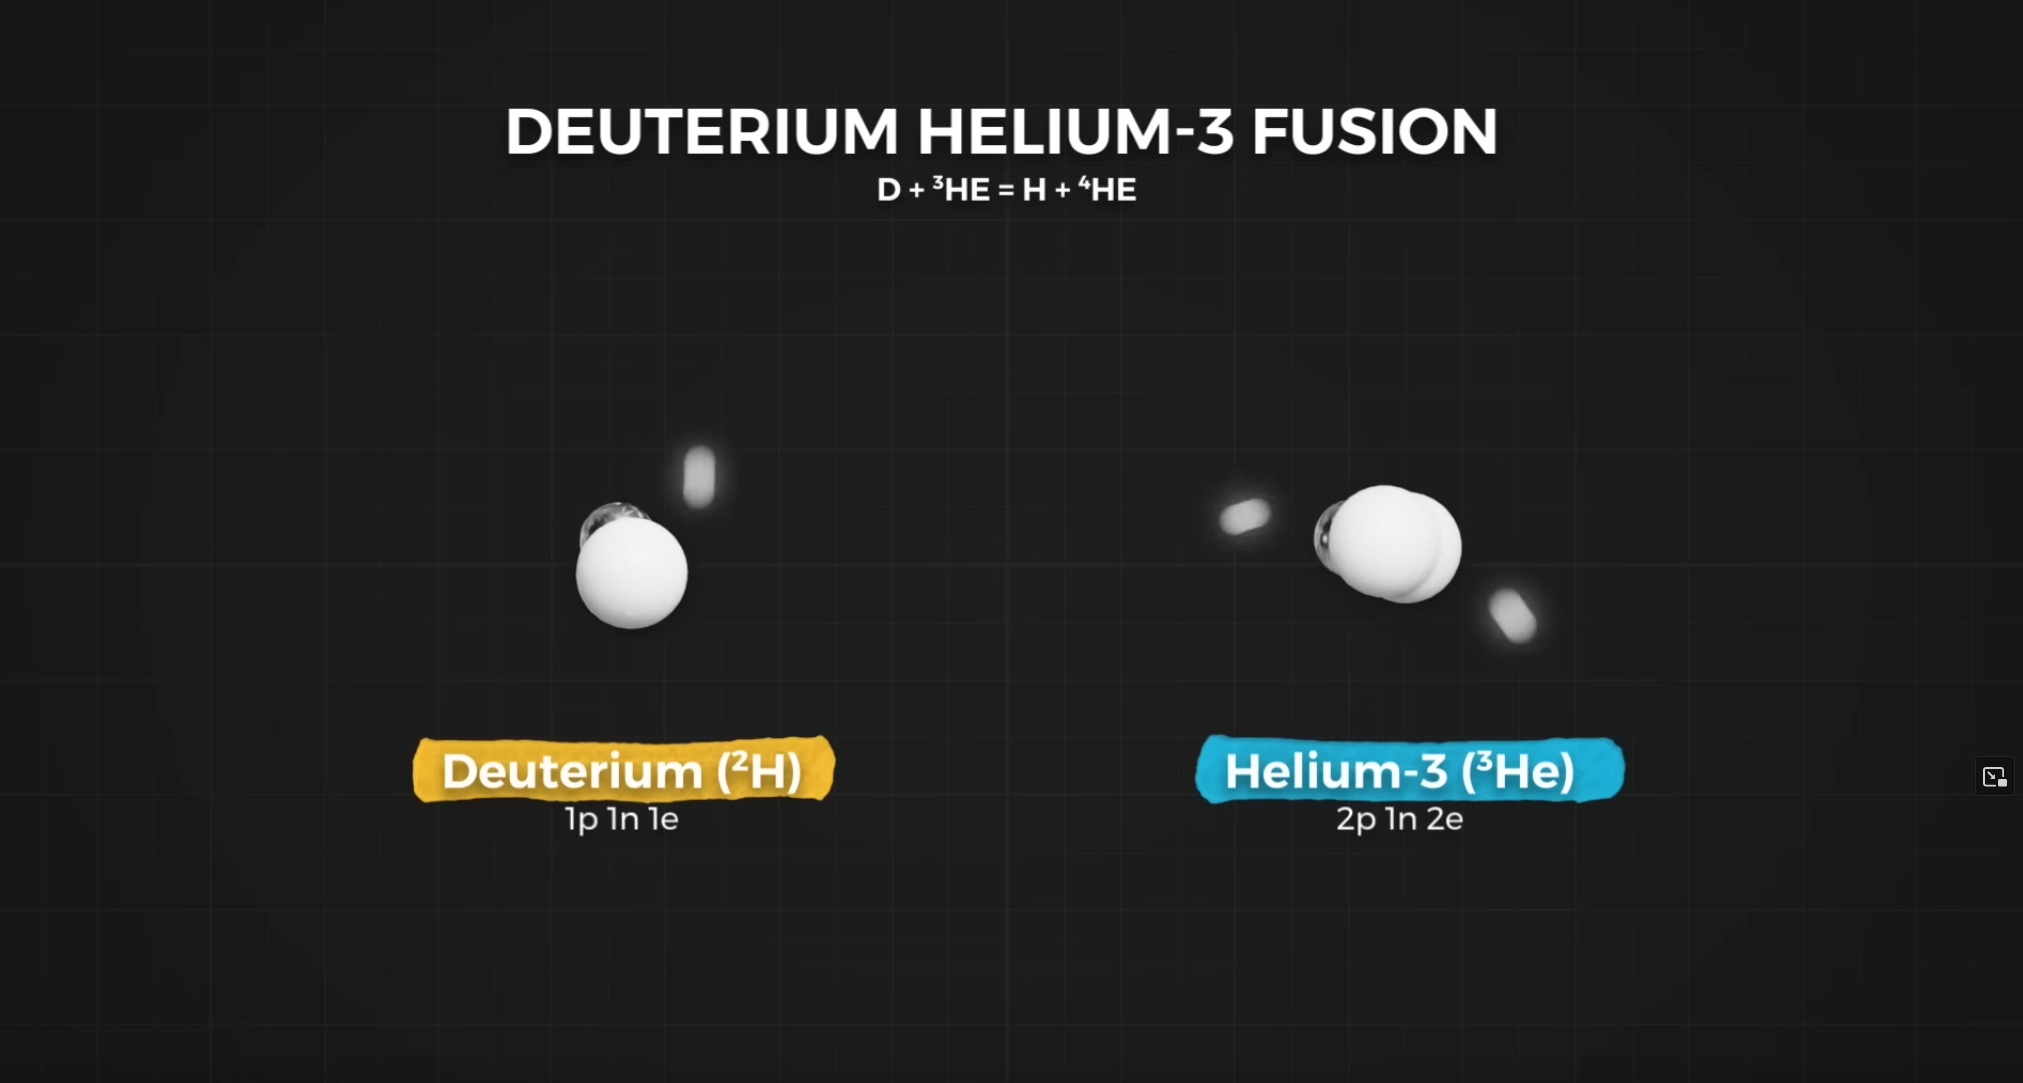
\includegraphics[scale=0.09]{d_h3_fusion.png}
            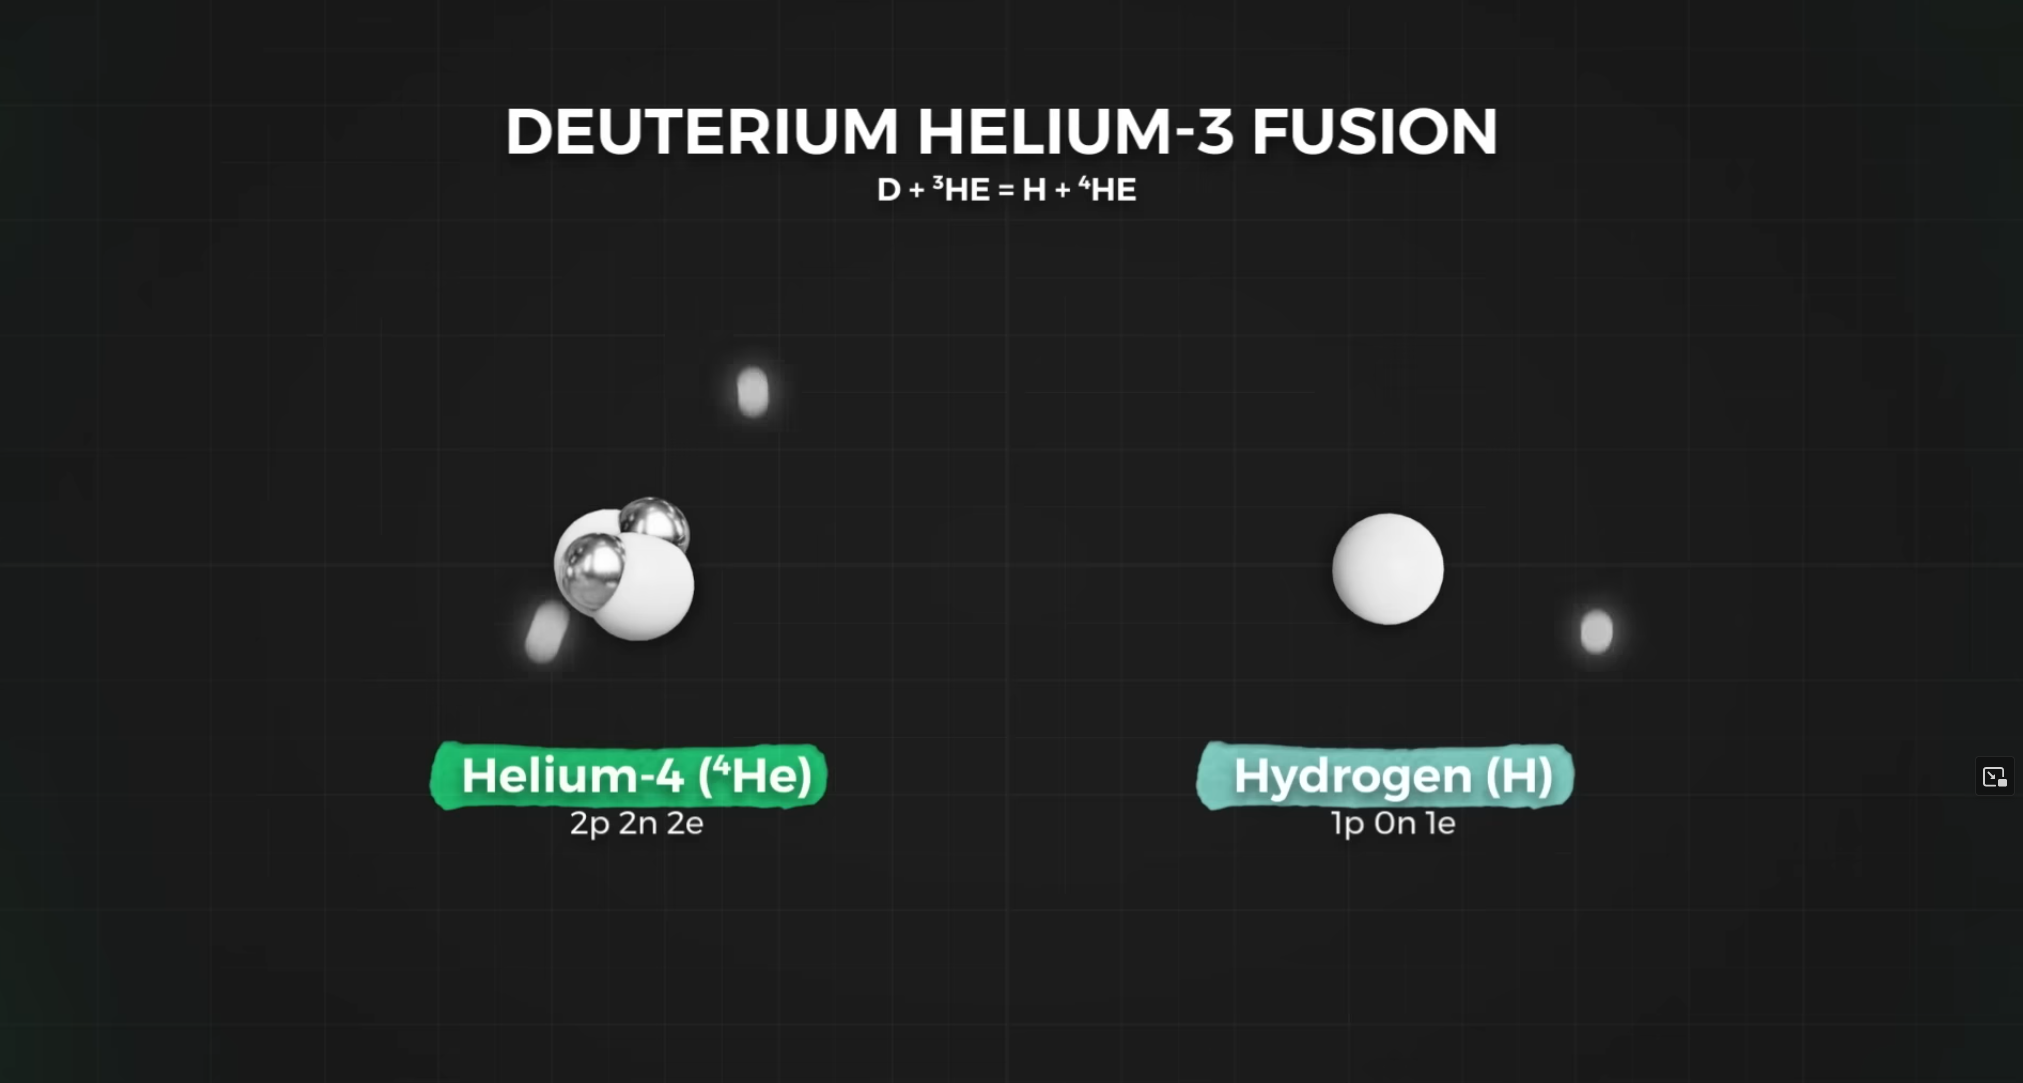
\includegraphics[scale=0.09]{d_h3_fusion_2.png}
        \end{figure}   
    \end{columns}
\end{frame}

\section{Célok a közeljövőben}
\begin{frame}
    \frametitle{Célok}
    \begin{itemize}
        \item Következő prototípus megépítése: Polaris 7. generáció
        \item Méret növelése: nagy gyro orbit miatt
        \item Áram termelés megvalósítása
    \end{itemize} 
\end{frame}
\subsection{Gyro Orbit probléma}
\begin{frame}
    \frametitle{Gyro Orbit}
    \begin{columns}
        \column{0.4\textwidth}
        \footnotesize
        \begin{itemize}
            \item Atomok pályája nagyobb mint elméletben
            \item Generátor falába csapódás valószínűsége megnő
        \end{itemize}
        \column{0.6\textwidth}
        \begin{figure}
            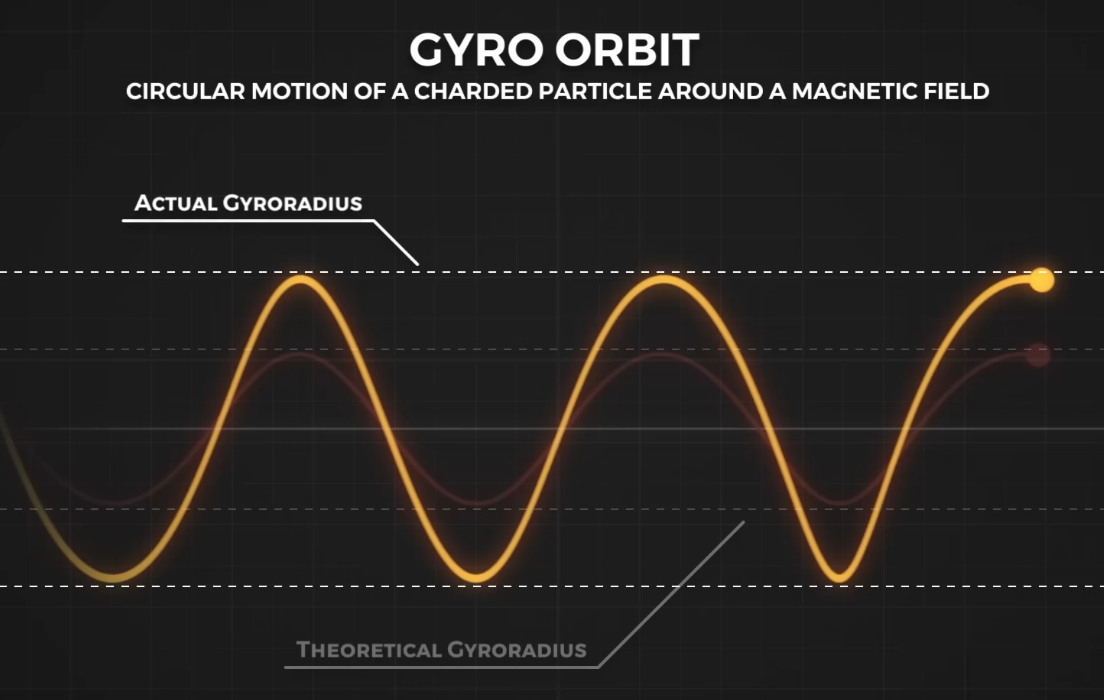
\includegraphics[scale=0.17]{gyro_orbit.png}
        \end{figure}    
    \end{columns}
    
\end{frame}

\section{Vége}
\begin{frame}
    \frametitle{Vége}
    \centering
    \Huge Köszönöm a figyelmet
\end{frame}

\section{Források}
\begin{frame}
    \frametitle{Források}
    \footnotesize
    \begin{itemize}
        \item \hypertarget{1}{\small[1]}\url{https://energyeducation.ca/encyclopedia/Nuclear_fusion_in_the_Sun}
        \item \hypertarget{2}{\small[2]}\url{https://en.wikipedia.org/wiki/Fusion_power}
        \item \hypertarget{3}{\small[3]}\url{https://www.iter.org/mach/Tokamak}
        \item \hypertarget{4}{\small[4]}\url{https://www.youtube.com/watch?v=_bDXXWQxK38&t=201s}
        \item \hypertarget{5}{\small[5]}\url{https://www.youtube.com/watch?v=G1vyMcqiVtA}
        \item \hypertarget{6}{\small[6]}\url{https://en.wikipedia.org/wiki/Field-reversed_configuration}
        \item \hypertarget{7}{\small[7]}\url{https://en.wikipedia.org/wiki/Neutral-beam_injection}
        \item \hypertarget{8}{\small[8]}\url{https://en.wikipedia.org/wiki/Plasma_beta}
        \item \hypertarget{9}{\small[9]}\url{https://en.wikipedia.org/wiki/Magnetic_helicity}
        \item \hypertarget{10}{\small[10]}\url{https://en.wikipedia.org/wiki/Aneutronic_fusion}
        \item \hypertarget{11}{\small[11]}\url{http://large.stanford.edu/courses/2022/ph241/ruiz2/}
    \end{itemize}
\end{frame}

\end{document}